 \documentclass[12pt]{article}
\usepackage[T2A]{fontenc}
\usepackage[utf8]{inputenc}       

\usepackage[english]{babel}
\usepackage{amsmath,amsfonts,amsthm,amssymb,amsbsy,amstext,amscd,amsxtra,multicol}
\usepackage{verbatim}
\usepackage{tikz}
\usetikzlibrary{automata,positioning}
\usepackage{multicol}
\usepackage{graphicx}
\usepackage[colorlinks,urlcolor=blue]{hyperref}
\usepackage[stable]{footmisc}
\usepackage{ dsfont }
\usepackage{wrapfig}
\usepackage{xparse}
\usepackage{ifthen}
\usepackage{bm}
\usepackage{color}
 \usepackage{subfigure}
 
\usepackage{algorithm}
\usepackage{algpseudocode}

\usepackage{xcolor}
\usepackage{hyperref}
\definecolor{linkcolor}{HTML}{799B03} % цвет гиперссылок
\definecolor{urlcolor}{HTML}{799B03} % цвет гиперссылок
 
%\hypersetup{pdfstartview=FitH,  linkcolor=linkcolor,urlcolor=urlcolor, colorlinks=true}

\newtheorem{theorem}{Theorem}[section]
\newtheorem{lemma}{Lemma}[section]

\DeclareMathOperator{\sign}{sign}
\DeclareMathOperator{\grad}{grad}
\DeclareMathOperator{\intt}{int}
\DeclareMathOperator{\conv}{conv}
\begin{document}

\section{Данные}

В собранной коллекции имелось 100 пар текстов. Каждая пара состоит из написанного в спокойном состоянии и написанного в фрустрированном состоянии одним и тем же человеком текстов. Для каждого текста были вычислены одинаковые признаки (всего призноков 198), и для каждой пары была вычислена разница между текстами.

Перед нами ставится задача кластеризировать эту разницу, т.е. мы хотим сгруппировать людей по схожести шаблона изменения состояния со спокойного на фустрированное. Более того, добавим ограничение, что нас интересует качественная схожесть, а именно, мы будем считать, что если есть два человека, у которых некоторый признак при переходе состояния увеличивается, то значение этого признака не изменяется качественно. Это обуславливает далее описываемую предобработку данных.

Во-первых, все признаки были отмасштабированы по максимальному абсолютному значению, что привело к тому, что все значения лежали на отрезке от -1 до 1, причем знак сохранился. Во-вторых, ко всем данным был применен модифицированный сигнум:

\begin{equation*}
\sign_\epsilon(x) = 
 \begin{cases}
   -1, \text{if } x < -\epsilon,\\
   0, \text{if } |x| \leq \epsilon,\\
   1, \text{if } x > \epsilon.
 \end{cases}
 ,
\end{equation*}
где $\epsilon$ - параметр. В наших экспериментах был выбран параметр, равный 0.2. Данный сигнум лучше обычного, поскольку он также показывает знак, но при этом принебрегает близкими к нулю значениями.

\section{Метод Кластеризации. Количество Кластеров.}

Перед основной кластеризацией был использован DBSCAN для поиска шумов и метрика Score Function для оценки качества того, насколько отделение шумов улучшает качество кластеризации по сравнению с качеством на одном кластере. Было получено, что DBSCAN не обнаружил таких шумов, удаление которых приводило бы к улучшению качества.

Зафиксируем следующую метрику качества кластеризации:

$$M(C) = \text{SF}(C) + \exp\left(-K\frac{\text{MaxSize}(C)-\text{MinSize}(C)}{N}\right),$$

где $\text{SF}$ - метрика для оценки качества кластеризации Score Function, $\text{MaxSize}, \text{MinSize}$ - размеры наибольшего и наименьшего кластеров, $N$ - количество кластеризируемых объектов, $K$ - количество кластера. Первое слагаемое этой метрики отвечает за качество, второе же слагаемое штрафует за несбалансированность классов, поскольку данная выборка имеет не достаточно большой размер, чтобы правильно в последствие оценить распределение значений признаков в маленьких кластерах.

Мы использовали различные известные алгоритмы кластеризации, при этом мы также варьировали количество кластеров в диапазоне от 1 до 10. Результаты Вы можете видеть на рис.\ref{choice}.

\begin{figure}[ht!]  
\centering 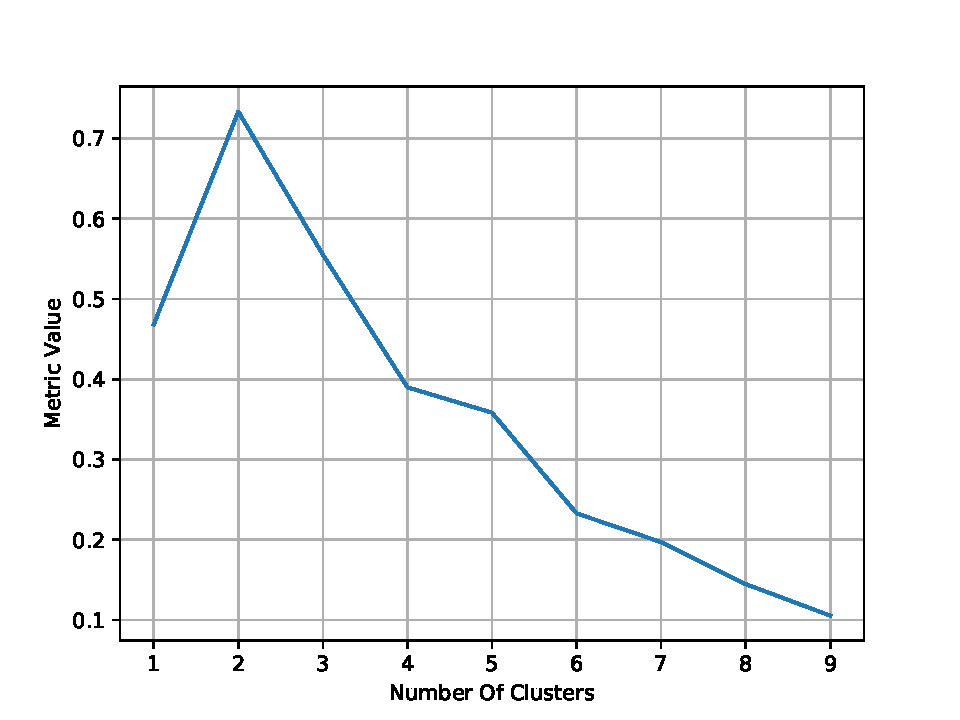
\includegraphics[width=1\linewidth]{Images/clusters_number.pdf}

\caption{....} \label{choice}
\end{figure}

Из результатов данного эксперимента следует, что наилучшим методом кластеризации является KMeans, причем оптимальным количеством кластеров является два. Далее мы будем использовать именно метод KMeans. Однако кроме кластеризации на два кластера, мы также рассмотрим и кластеризацию на 4, как на наибольшее количество кластеров, для которого значение метрики упало менее, чем в два раза.

Крому того, что нам нужно кластеризовать, нам следует выделить наиболее различающиеся признаки у кластеров. Мы это делаем тривиальным образом: высчитать среднее значение всех признаков для каждого кластера, получить разницу между средними для всех пар кластеров, оценить информативность, как максимальную по всем парам разницу для каждого признака, отранжировать их по информативности и выбрать все, у которых информативность больше 70$\%$ от максимальной.

\section{Кластеризация на два кластера}
\label{sec:cluster}

Наиболее различающиеся признаки получаются следующие (записаны в порядке возрастания):

\begin{itemize}
\item Коэффициент Трейгера
\item Коэффициент опредмеченности действия (кол. глаголов / кол. существительных)
\end{itemize}

Посмотрим на распределения значений для соответствующих признаков, причем мы будем смотеть на отмасштабированные значения. Для каждого признака мы взяли интервал [-1,1], в котором лежат значения этого признака, разбили его на 10 частей, посчитали для каждого кластера количество объектов со значением этого признака в соответствующей части и нормализовали полученные распределения (сделали так, чтобы интеграл по всему интервалу был равен единице). Соответствующие гистограммы Вы можете видеть на \ref{hist1}.

\begin{figure}[ht!]  
\vspace{-4ex} \centering \subfigure[]{
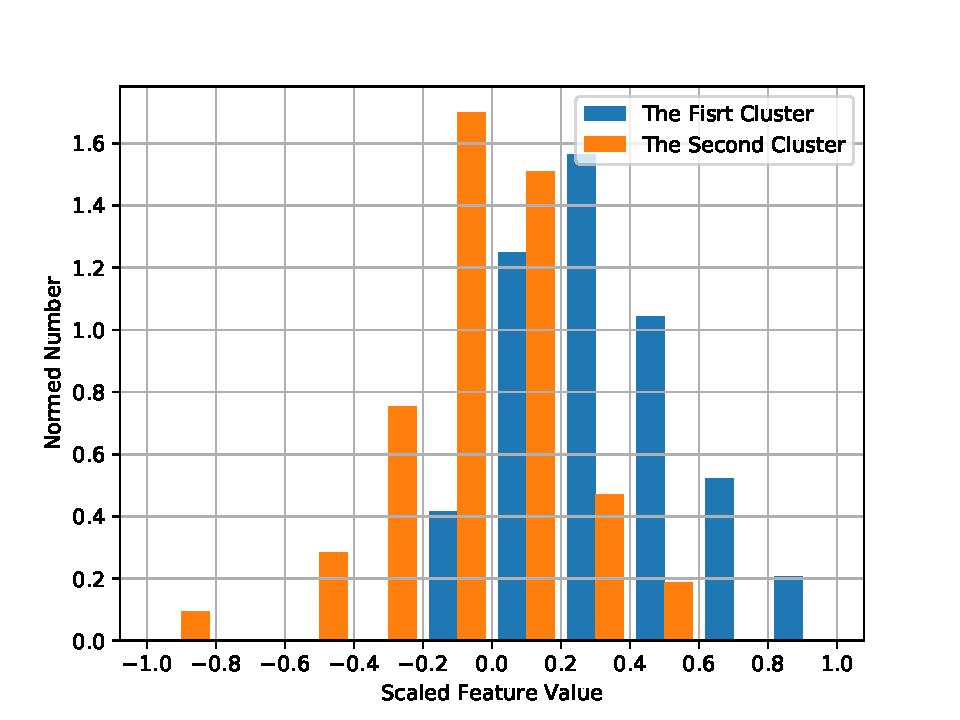
\includegraphics[width=0.4\linewidth]{Images/Signum/1.pdf} \label{1} }  
\hspace{2ex}
\subfigure[]{
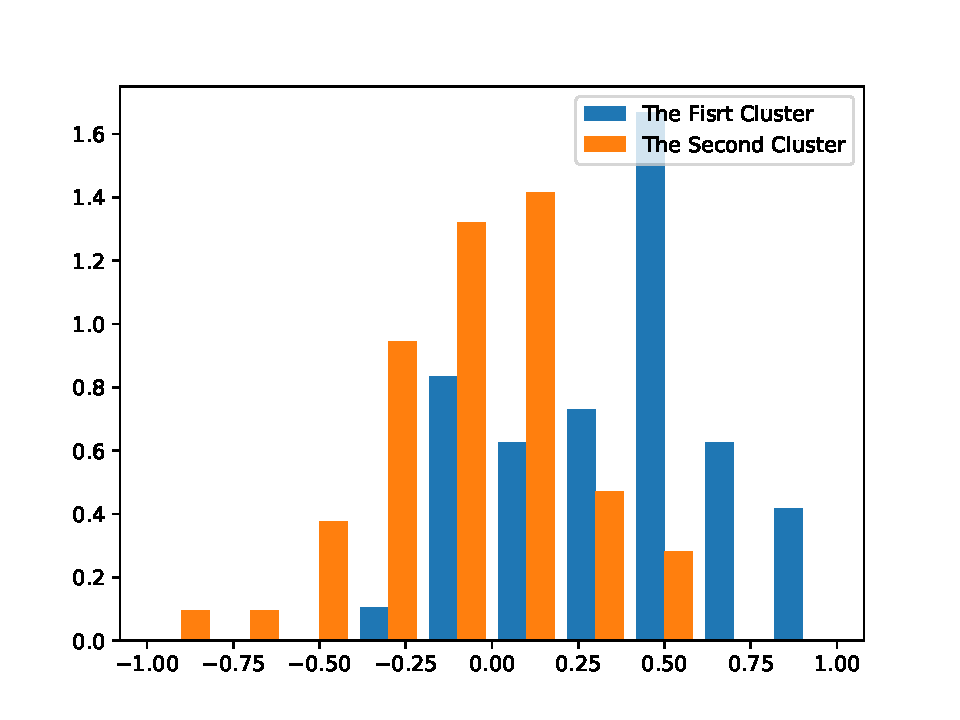
\includegraphics[width=0.4\linewidth]{Images/Signum/2.pdf} \label{2} }  

\caption{Сравненение распределения для наиболее различающихся признаков: \subref{1} Коэффициент Трейгера; \subref{2} Коэффициент опредмеченности действия (кол. глаголов / кол. существительных).} \label{hist1}
\end{figure}

\section{Кластеризация на четыре кластера}
\label{sec:cluster}

Наиболее различающиеся признаки получаются следующие (записаны в порядке возрастания):

\begin{itemize}
\item Доля глаголов 1 лица
\item Сем. связь: QNT
\item Сем. роль: адресат
\item Число знаков пунктуации / Число слов
\item Средняя длина слов (в количестве символов)
\item Доля глаголов прошедшего времени
\item Коэффициент Трейгера
\item Словарь: Лексика положительной рациональной оценки и ментальных действий
\end{itemize}

Посмотрим на распределения значений для соответствующих признаков, причем мы будем смотеть на отмасштабированные значения. Для каждого признака мы взяли интервал [-1,1], в котором лежат значения этого признака, разбили его на 10 частей, посчитали для каждого кластера количество объектов со значением этого признака в соответствующей части и нормализовали полученные распределения (сделали так, чтобы интеграл по всему интервалу был равен единице). Соответствующие гистограммы Вы можете видеть на \ref{hist2} и \ref{hist3}.

\begin{figure}[ht!]  
\vspace{-4ex} \centering \subfigure[]{
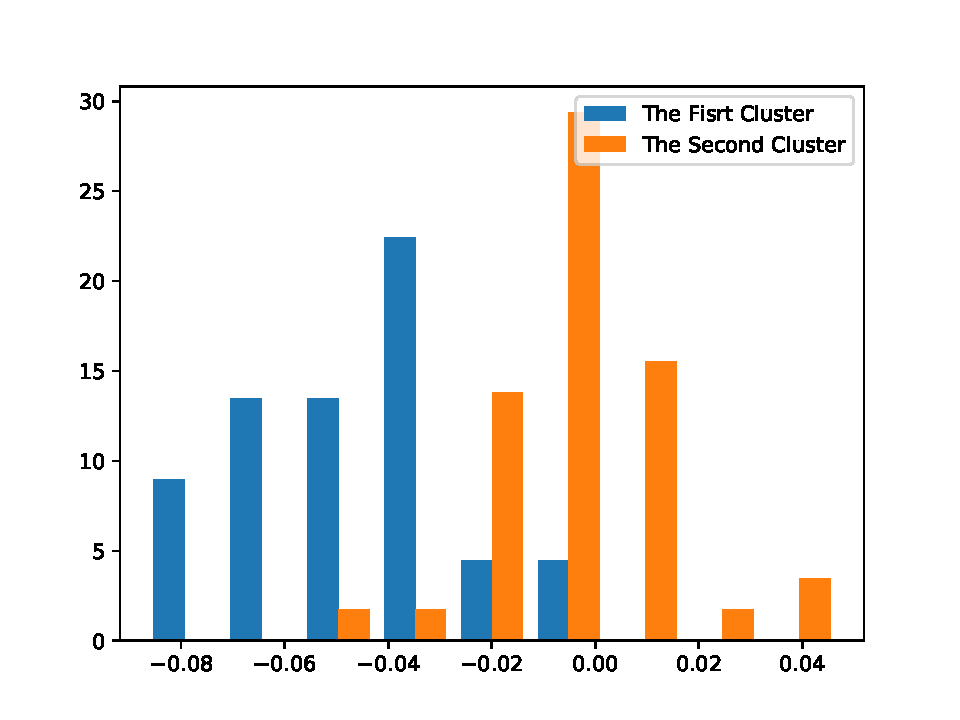
\includegraphics[width=0.4\linewidth]{Images/ManyClusters/1.pdf} \label{1} }  
\hspace{2ex}
\subfigure[]{
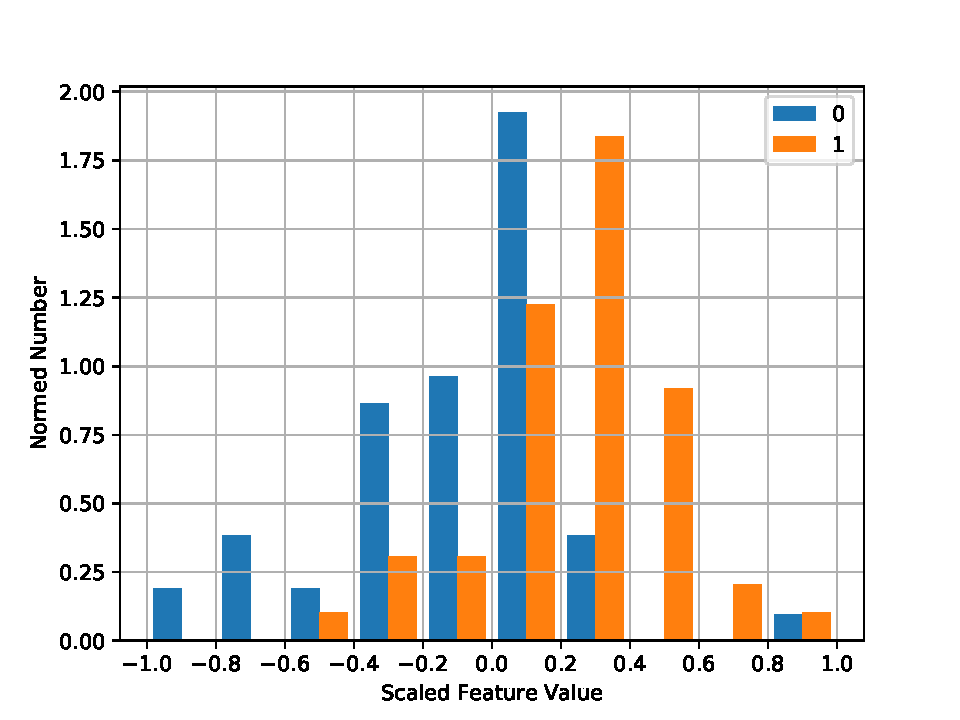
\includegraphics[width=0.4\linewidth]{Images/ManyClusters/2.pdf} \label{2} }  
\vspace{2ex} \centering \subfigure[]{
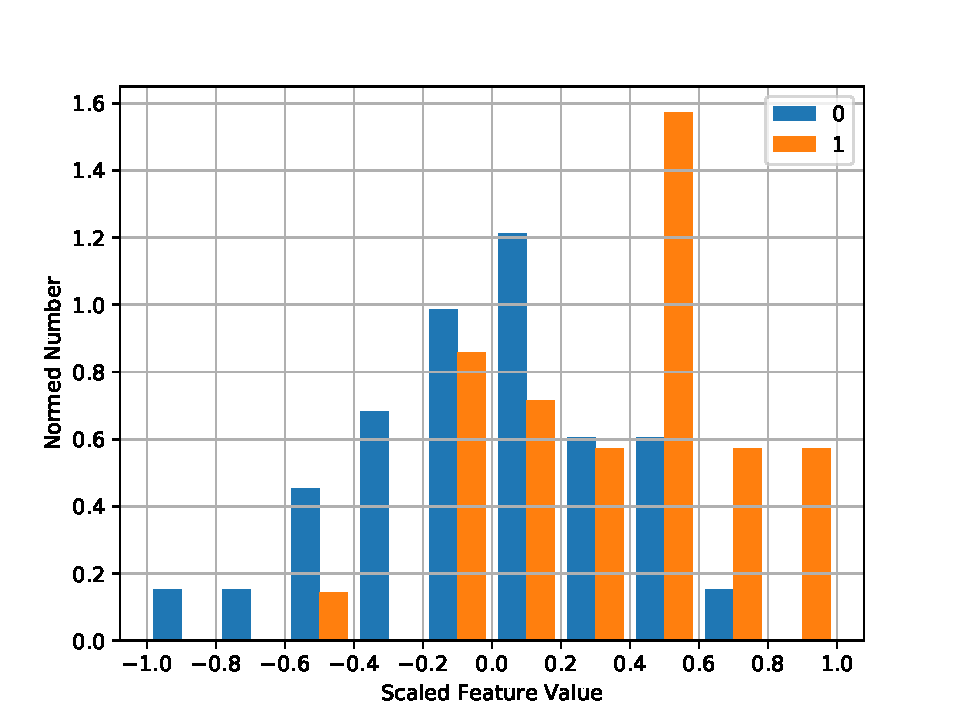
\includegraphics[width=0.4\linewidth]{Images/ManyClusters/3.pdf} \label{3} }  
\hspace{2ex}
\subfigure[]{
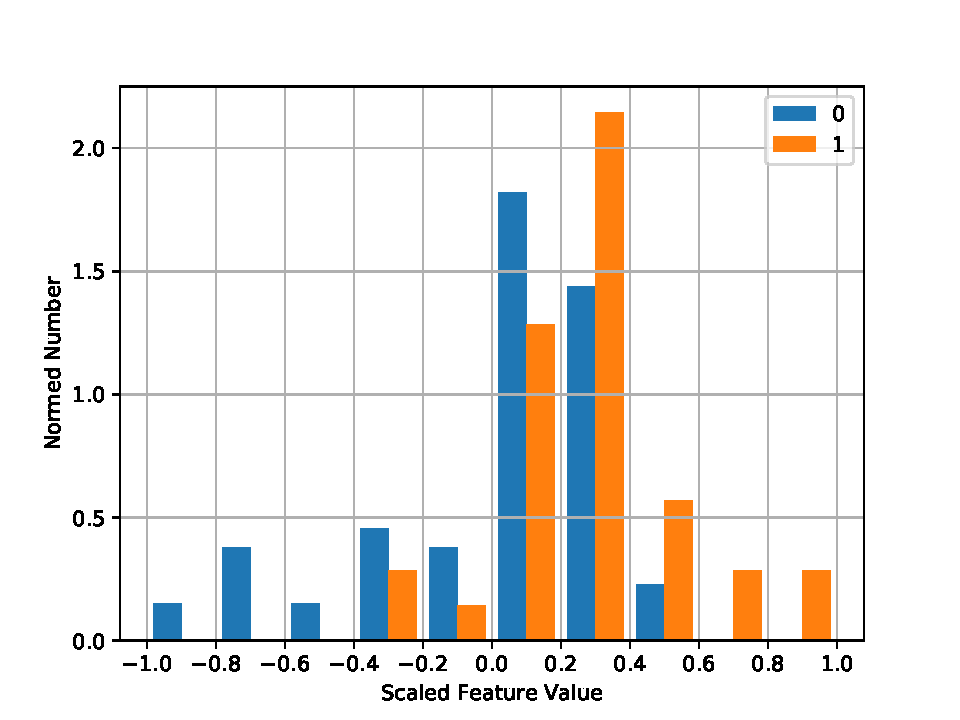
\includegraphics[width=0.4\linewidth]{Images/ManyClusters/4.pdf} \label{4} }  
\caption{Сравненение распределения для наиболее различающихся первых четырех признаков: \subref{1} Доля глаголов 1 лица; \subref{2} Сем. связь: QNT; \subref{3} Сем. роль: адресат; \subref{4} Число знаков пунктуации / Число слов.} \label{hist2}
\end{figure}

\begin{figure}[ht!]  
\vspace{-4ex} \centering \subfigure[]{
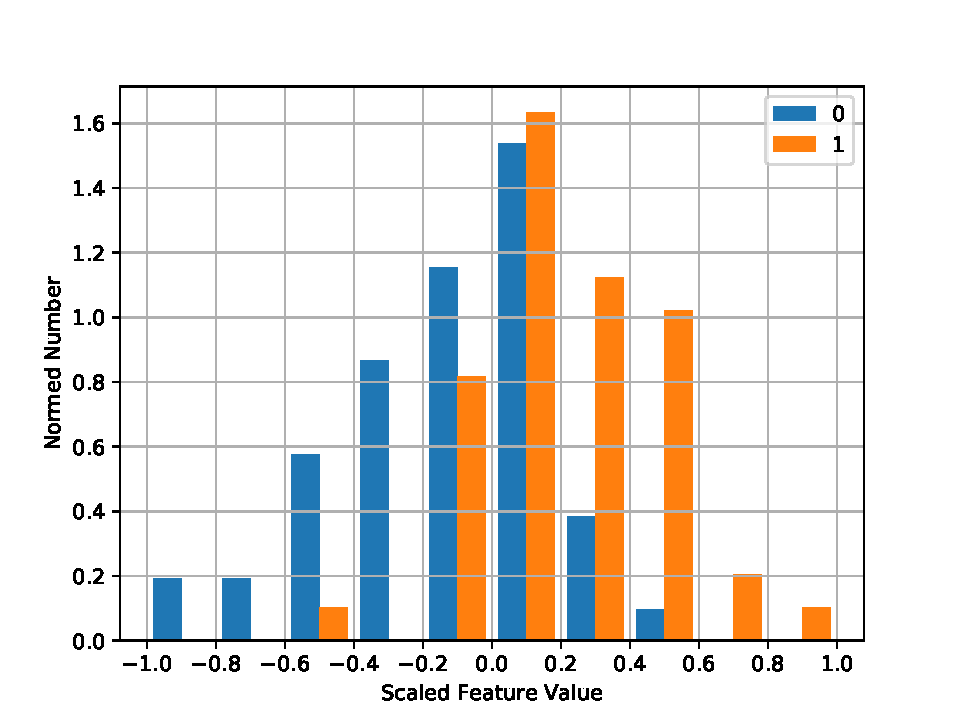
\includegraphics[width=0.4\linewidth]{Images/ManyClusters/5.pdf} \label{5} }  
\hspace{2ex}
\subfigure[]{
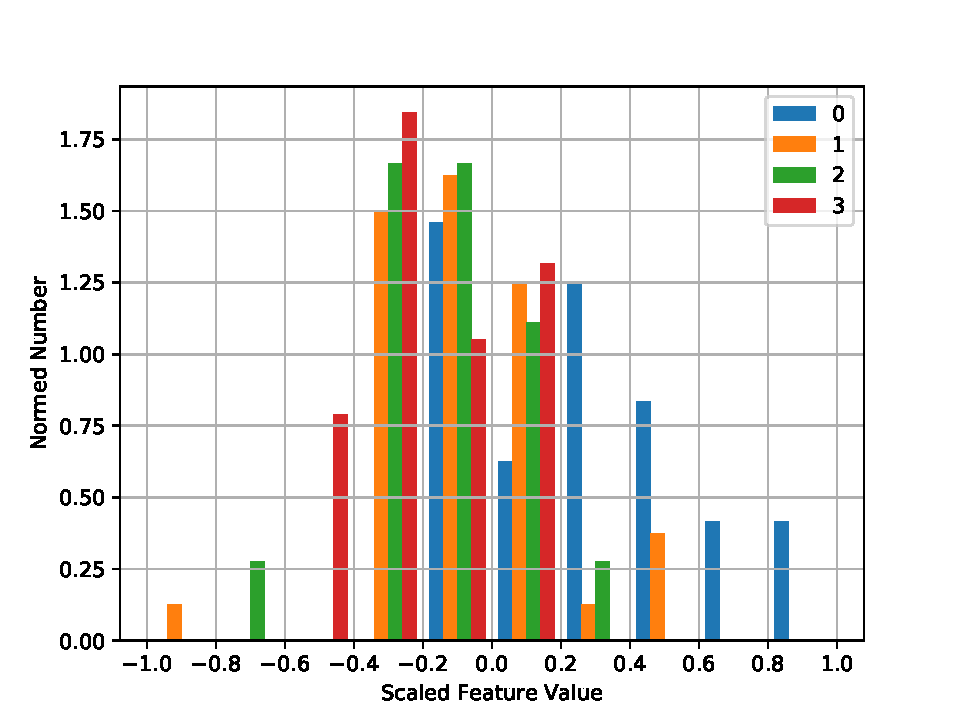
\includegraphics[width=0.4\linewidth]{Images/ManyClusters/6.pdf} \label{6} }  
\vspace{2ex} \centering \subfigure[]{
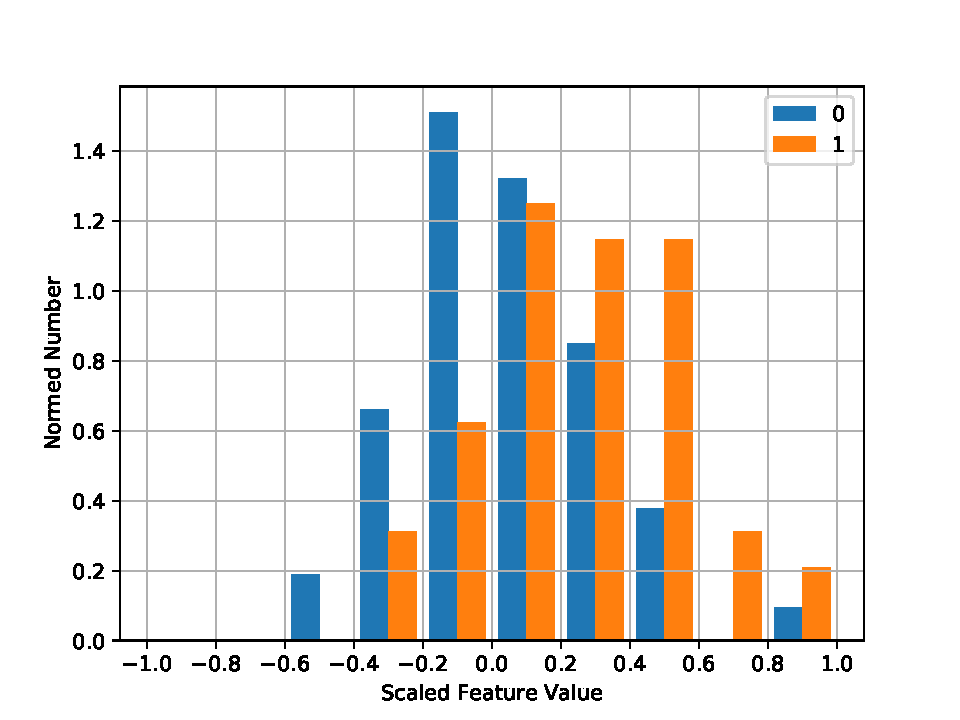
\includegraphics[width=0.4\linewidth]{Images/ManyClusters/7.pdf} \label{7} }  
\hspace{2ex}
\subfigure[]{
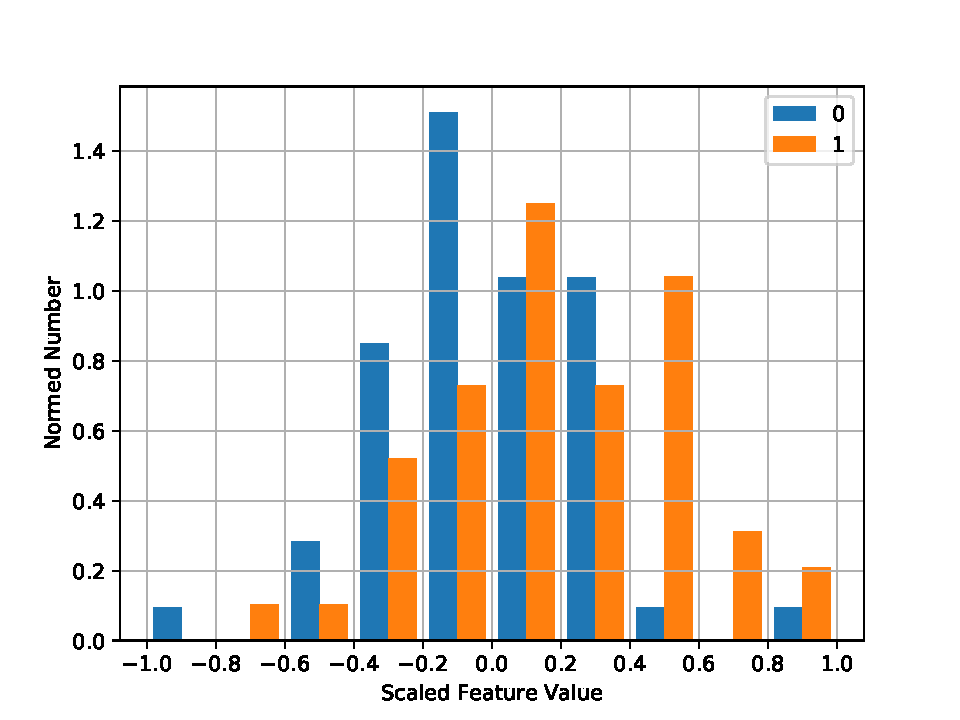
\includegraphics[width=0.4\linewidth]{Images/ManyClusters/8.pdf} \label{8} }  
\caption{Сравненение распределения для наиболее различающихся последних четырех признаков: \subref{5} Средняя длина слов (в количестве символов); \subref{6} Доля глаголов прошедшего времени: QNT; \subref{7} Коэффициент Трейгера; \subref{8} Словарь: Лексика положительной рациональной оценки и ментальных действий.}  \label{hist3}
\end{figure}

\end{document}


